\chapter{Selbstführung}
Führen von Menschen = mit Menschen Zielen erreichen. Man muss Menschen mögen. Die wichtigste Person, welche geführt werden muss, bin ich selbst. Dafür brauchts Selbsterkentniss, Selbst-Akzeptanz und Selbst-Steuerung.

Oft setzen wir uns eins Ziel (auf MEP lernen) und verhalten uns nicht zielführend (in Badi statt Lernen). Somit muss noch etwas anderes auf unseren Verstand Einfluss nehmen.

\paragraph{Glaubensregeln}
Überlieferungen, kultureller Rahmen der Gesellschaft, eigene Lebenserfahrungen. Diese gehören zur Sammlung unserer Überzeugungen, welche wir unbewusst aufnehmen. Sind uns diese Regeln jedoch bewusst, können wir diese löschen, ändern oder ersetzen.

\section{Sie kennen die Bedeutung des Unterbewusstseins für unser Verhalten und wie man damit interagiert}

\paragraph{Erkentnisse zur Selbststeuerung}
\begin{itemize}
	\item Etwas mit dem rationalen Verstand zu wollen, genügt nicht zur wirksamen Zielerreichung
	\item Es gibt zwei relevante Akteure, die Einfluss auf mein Verhalten nehmen: Mein rationaler Verstand und mein Unterbewusstsein. (2 Optionen - Kampf gegen UB mit Disziplin und Verbissenheit oder Zusammenarbeit mit UB)
\end{itemize}

\begin{figure}[h!]
	\centering
	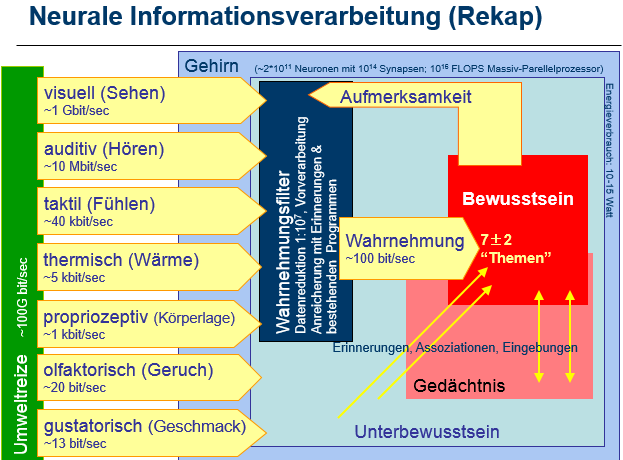
\includegraphics[width=0.7\linewidth]{fig/neurale-informationverarbeitung}
	\caption{}
	\label{fig:neurale-informationverarbeitung}
\end{figure}

Das Bewusstsein arbeitet langsam (>900ms) und nur unter guten Bedingungen. Es beobachtet und interpretiert Entscheide für das UB (Pressesprecher des UB). Das UB reagiert schnell (<200ms) und in jeder Lebenslage. Beide arbeiten gleichzeitig und konkurrierend, sie können sich widersprechen. 

Erfolg = UB und Bewusstsein haben das selbe Ziel.

UB ist zu 100 Prozent ehrlich. Nimmt nie Rücksicht auf irgendetwas. Es ist fantasielos und nimmt alles wörtlich.

\paragraph{Steuerungsmöglichkeiten für das UB}
\begin{itemize}
	\item Gezielte Instruktion durch kluge Zielsetzung. Das UB hört mit. Durch gezielten Input kann ich die richtigen Programme im UB aufrufen.
	\item Re-Programmierung. UB funktioniert auf Basis gespeicherten Glaubenssätzen = kondensierte Erfahrungen = Programme. Ändern die Glaubenssätze, ändern die Programme dauerhaft! 
\end{itemize}

\paragraph{Wie programmiere ich das UB?}
Gut Frage Sherlock! Reden (einfach), Bild vorstellen (wirkungsvoll), körperlich erleben.

\paragraph{Wie weiss ich was das UB will? Wie es momentan programmiert ist?}
First of all - es kann nicht reden! Über Körperreaktionen, Gedankenblitzer, alle Sofortreaktionen.

\paragraph{Somatische Marker}
Jede körperliche Reaktion, jedes mentale Bild, Szene, Erinnerung die unmittelbare (Millisekundenbereich) auf die Frage/den Begriff wahrnehmbar wird, ist ein somatischer Marker. Bsp: Kribbeln im Bauch, Erregung, Kneifen, plötzliche Schmerzen, Gefühl von Hunger/Durst usw. Dieses Gefühl kann positiv oder negativ wahrgenommen werden. Darum gibt es zwei Skalen, eine für das positive Gefühl und eine für das negative Gefühl. Das emotionale Gewischt (positiv = Lust/negativ = Abscheu) welches man empfindet wird als Wert in den beiden Skalen eingetragen. Den Wert bestimmt man selbst.

\section{Sie wissen, welche Eigenschaften eine wirksame Zielformulierung umfasst}
\label{sec:how-to-be-successful-with-ub}

\begin{description}
	\item[1. Schritt - Satz was will ich] Ich gebe Instruktionen ans UB in Form von Sätzen, welche eine Zielformulierung beinhalten. Zielsatz formulieren, Zielsatz lesen. Welche Gefühle kommen dabei hoch? Somatische Marker +/- pro Wort bestimmen. Wenn weniger als -0/+70, Wort stärken.
	\item[2. Schritt - Motivation prüfen] 5 Gründe warum ich das Ziel erreichen will. Alle eigenen Gründe markieren, streichen aller fremden Gründe.
	\item[3. Schritt - Wirksamkeits-Check] Autonomie: Ich kann das Ziel selbständig erreichen. Wirksame Formulierung überprüfen (Erreichungsziel, keine Negation, keine Vergleiche, keine Relativierung, keine Zwänge, im Hier und Jetzt). Formulierung hat einen Energie-Pegel von -0/+70. 
\end{description}
Jetzt ist die Macht mit Dir! Das UB ist programmiert und unterstützt dich.
Nonplusultra: Das Ziel mit einer Metapher verknüpfen. Das UB arbeitet nun auch ohne meine Aufmerksamkeit. Eine Zielformulierung ist dann besonders wirksam, wenn sie folgende Eigenschaften zeigt:

\begin{enumerate}
	\item Ein Satz mit Somatischen Markern von -0/+70 oder besser
	\item Sie basiert auf einem guten eigenen Grund (Keine Fremdmotivation)
	\item Ich kann es unabhängig von anderen erreichen (Autonomie)
	\item Es geht darum, etwas zu erreichen, nicht, etwas zu vermeiden
	\item Es ist aktiv formuliert, d.h. 
	\begin{itemize}
		\item keine Verneinungen
		\item keine Vergleiche
		\item keine Relativierungen
		\item als erreichten Zustand in der Gegenwart (nicht ich werde sondern ich bin)
		\item keine Begriffe wie «soll», «muss», sondern «will» oder «kann». Bei Bedarf kann ich die Formulierung «ich beschliesse» oder «ich entscheide» verwenden.
	\end{itemize}
\end{enumerate}


\section{Sie wissen, wie ein Auftrag an das Unterbewusstsein (Programmierung) formuliert sein muss, damit es auch tatsächlich wie gewünscht wirkt.}

Siehe dazu \ref{sec:how-to-be-successful-with-ub}
